\documentclass[tikz]{standalone}
\begin{document}
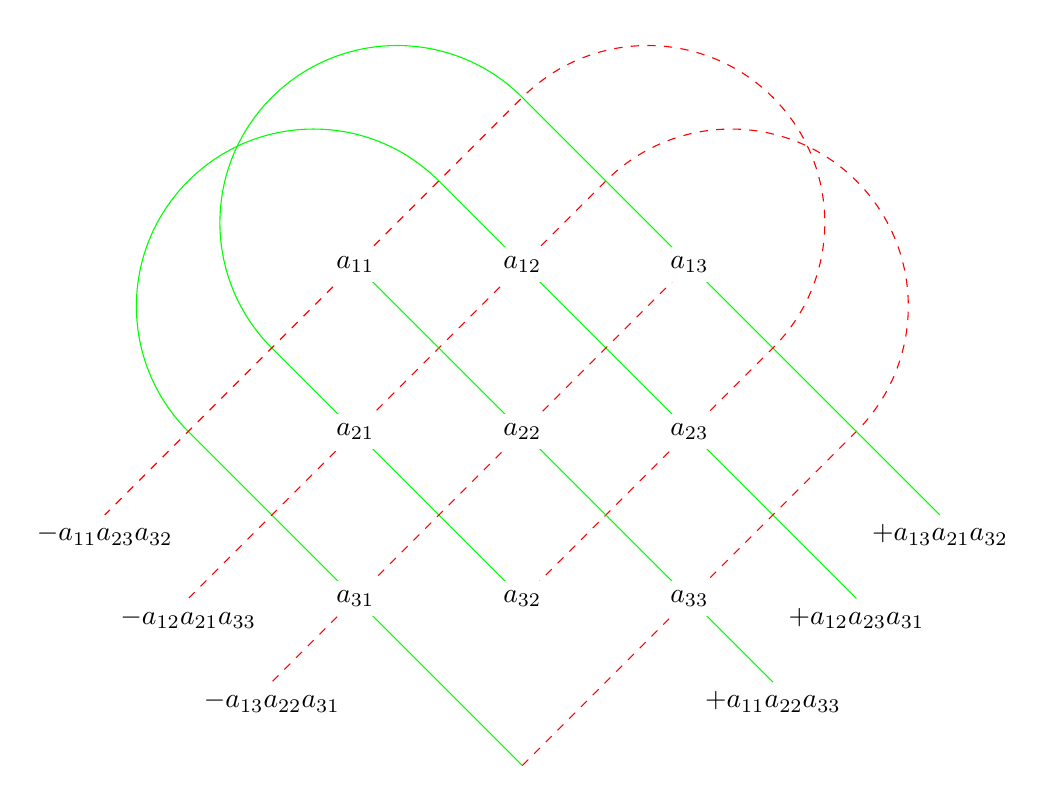
\begin{tikzpicture}[scale=1.5]
\tikzset{
  temp/.cd,
    s opt/.store in=\solidlineopt, s opt={draw=green},
    s path/.store in=\solidlinepath, s path=,
    s end opt/.store in=\solidlineendopt, s end opt={below},
    s end text/.store in=\solidlineendtext, s end text=,
    d opt/.store in=\dashedlineopt, d opt={draw=red,dashed},
    d path/.store in=\dashedlinepath, d path=,
    d end opt/.store in=\dashedlineendopt, d end opt={below},
    d end text/.store in=\dashedlineendtext, d end text=,
}
\def\linesdraw#1{
  \begingroup
    \tikzset{temp/.cd,#1}
    \edef\tempcmd{
      \noexpand\begin{scope}
        \noexpand\draw[\solidlineopt]\solidlinepath node[\solidlineendopt]{\solidlineendtext};
      \noexpand\end{scope}
      \noexpand\begin{scope}
        \noexpand\draw[yscale=-1,rotate=-90,\dashedlineopt]
          \dashedlinepath
          node[\dashedlineendopt]{\dashedlineendtext};
      \noexpand\end{scope}
    }
    \tempcmd
  \endgroup
}
\begin{scope}[rotate=-135]
    \foreach \i/\j/\k in {
        {(4,4)--(4,0)arc(0:-180:1.5)--(1,5)}/{$+a_{12}a_{23}a_{31}$}/{$-a_{12}a_{21}a_{33}$},
        {(3,3)--(3,0)arc(0:-180:1.5)--(0,5)}/{$+a_{13}a_{21}a_{32}$}/{$-a_{11}a_{23}a_{32}$},
        {(2,0)--(2,5)}/{$+a_{11}a_{22}a_{33}$}/{$-a_{13}a_{22}a_{31}$}
    }{
        \linesdraw{
        %  s opt=,
        s path={\i},
        %  s end opt={},
        s end text={\j},
        %  d opt=,
        d path={\i},
        %  d end opt={},
        d end text={\k},
        }
    }
\end{scope}
\begin{scope}[yscale={-sqrt(2)},xscale={sqrt(2)},shift={(-2,0)}]
\foreach \i in {1,2,3}{
    \foreach \j in {1,2,3}{
        \node [fill=white] at(\i,\j){$a_{\j\i}$};
    }
}
\end{scope}
\end{tikzpicture}

\end{document}